\chapter{Framework for Ad-hoc Social Networks Middleware}\label{Chap3}
\echapter{Framework for Ad-hoc Social Networks Middleware}

\section{Introduction}\label{Chap3_01}
\esection{Introduction}
The improved computational and storage capacity of mobile devices now makes them capable to be applied in broad range of applications. In addition to that, the incorporation of sensing technologies and better connectivity has made it easier to support pervasive systems and allow users to manage their data and share information. Data collected from these mobile (smart) devices has recently fascinated an increase interest in the scientific and academic research community as compared to the traditional way of sensing user activities. Sensor data collected and processed using intelligent technologies is expected to provide much richer user information such as mobility efficiently (less cost, time and personal bias). However, current frameworks for wireless networks provide limited support for middleware levels such as social awareness, requiring designers and developers to deal with low level layers such as sensing and analyzing data.

To address this problem, we have presented an ASNET middleware framework to support the requirements for designing protocols/algorithms of ad-hoc social applications such as pervasive conference systems. The presented framework ensures that designers and developers can work at the higher levels of the framework, without dealing with the low level mechanisms such as mobile crowdsensing, learning and acquisition. Instead, protocols or algorithms can be designed based on the available user social and mobility information from the modeled social graph using social network analysis techniques. Therefore, the presented framework supports often used components/sub-components that can facilitate and speed up the proposal of new innovative middleware protocols.

\section{Formal Framework and Components}\label{Chap3_02}
\esection{Formal Framework and Components}
\begin{figure}[t]
\begin{center}
  \begin{tabular}{c}
  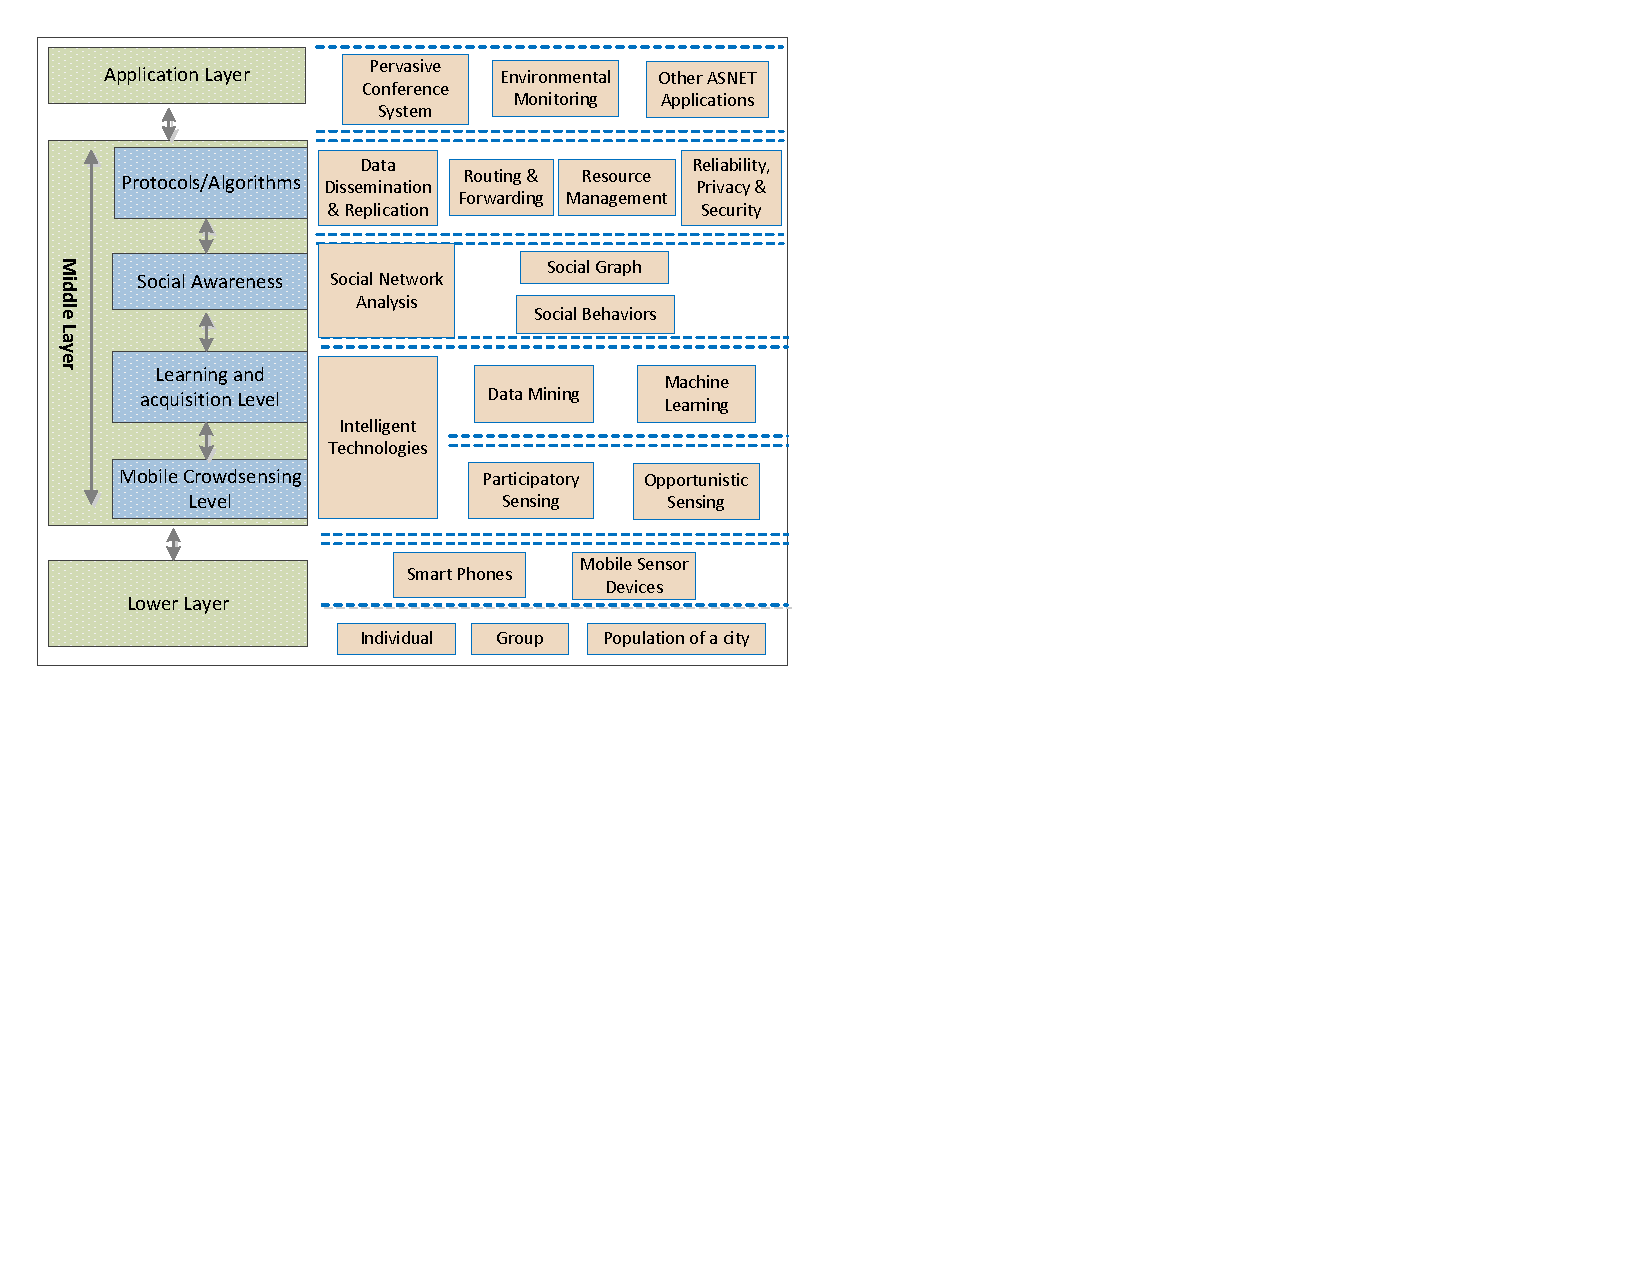
\includegraphics[width=0.8\textwidth]{Chap3-Fig4.pdf}
  \end{tabular}
  \caption{A general ASNETs system framework which integrates layers from sensing level to application level.}
\end{center}
\end{figure}

To introduce this emerging field and to achieve the design of efficient protocols to support upper layer applications, we propose an ASNET system framework that integrates different layers as depicted in Fig. 3.1. The different sensing systems in the mobile crowdsensing layer operate at multiple low level scales, enabling everything from individual to community (group) and then to global (population) sensing using smart phones and mobile sensor devices. The next step is to extract information from the sensors using intelligent technologies. These occur either directly on the smart device or in the mobile cloud. Social awareness will be achieved using social graph by analyzing the collected information through learning and acquisition layer. Once social information is available from the social awareness layer, it will be a valuable input to design the protocols/algorithms. Thus, this layer brings essential issues for ASNETs middleware. In what follows, we decompose the main different components of an ASNET middleware system and briefly touch on these components and the corresponding functions.

\subsection{Mobile Crowdsensing}\label{Chap3_02_01}
\esubsection{Mobile Crowdsensing}
The mobile crowdsensing component (Fig. 3.2) is responsible for sensing and sharing data observations from the lower layer (different scales; individual, group or community) that are relevant to user behavior with respect to the type of protocol/algorithm to be designed and for periodically reporting them to the learning and acquisition component. Usually, the mobile crowdsensing would operate on individuals with smart phones and sensing devices that collectively sense and share data to measure and map phenomena of different activities such as interest. Based on the type of activities being observed, lower sensing level can be broadly categorized as individual and community sensing.
\begin{figure}[t]
\begin{center}
  \begin{tabular}{c}
  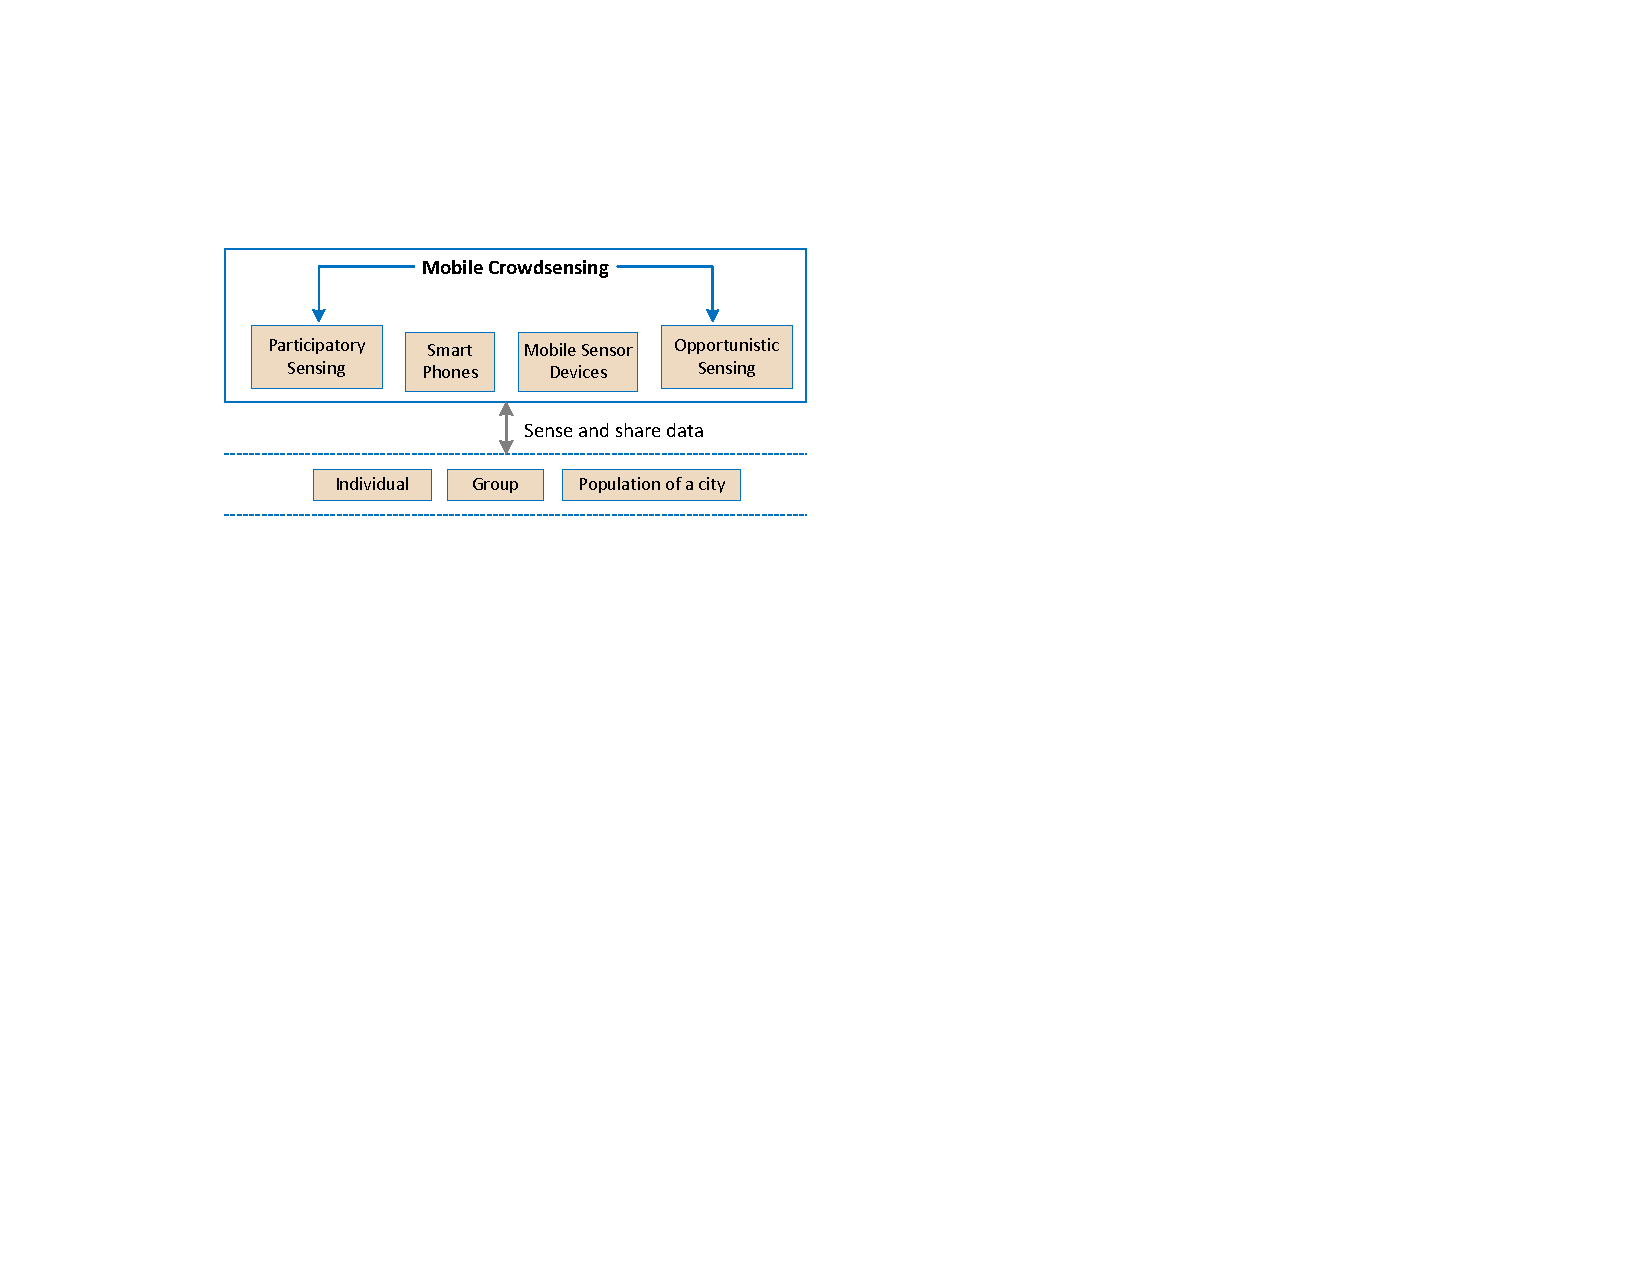
\includegraphics[width=0.65\textwidth]{Chap3-Fig1.pdf}
  \end{tabular}
  \caption{The mobile crowdsensing component.}
\end{center}
\end{figure}

In individual sensing, the activities pertaining to an individual; for example, the movement patterns of an event such as conference attendant for keeping personal records or facilitating the event. Another example of individual sensing is one that observes the transportation means of a person to track his or her recent destinations. Different from individual sensing, community sensing refers to the observation of large-scale activities that cannot simply be quantified by a single person. For example, pervasive conference management systems may require attendants activity interest monitoring and research keywords monitoring. These activities can be accurately measured only when many attendants provide their interest and research keyword information, which are then aggregated dynamically to determine the interest and research keyword in a particular conference.

As shown in Fig. 3.2, the sensing could be participatory sensing~\cite{OOmokaro2012} or opportunistic sensing~\cite{GSTuncay2013}. In participatory sensing, there is an active participation of users to contribute sensor data related to an activity at different levels. Opportunistic sensing is more autonomous, and there is minimal participation of users. Therefore, mobile crowdsensing spans a wide spectrum of user involvement, with participatory sensing and opportunistic sensing at the two ends~\cite{RKGanti2011}. Compared to traditional sensing mechanisms, mobile crowdsensing has a number of unique characteristics that bring both new opportunities for the design of ASNET middleware protocols. Firstly, smart phones or mobile sensor devices have significantly more communication, computation, and storage resources than traditional sensors, and are equipped with broad sensing capabilities. Secondly, users carry these devices wherever they go and whatever they do which makes it to be deployed in this research field. By employing these devices, we believe that it is possible to design middleware protocols and algorithms efficiently in terms of cost and time. For example, in a conference hall, instead of installing floor cameras and detectors, it is possible to collect participants' data and detect movement levels using smart phones carried by the attendants in such a way that it reduces the cost of specialized sensing infrastructure deployment.

\subsection{Learning and Acquisition}\label{Chap3_02_02}
\esubsection{Learning and Acquisition}
\begin{figure}[t]
\begin{center}
  \begin{tabular}{c}
  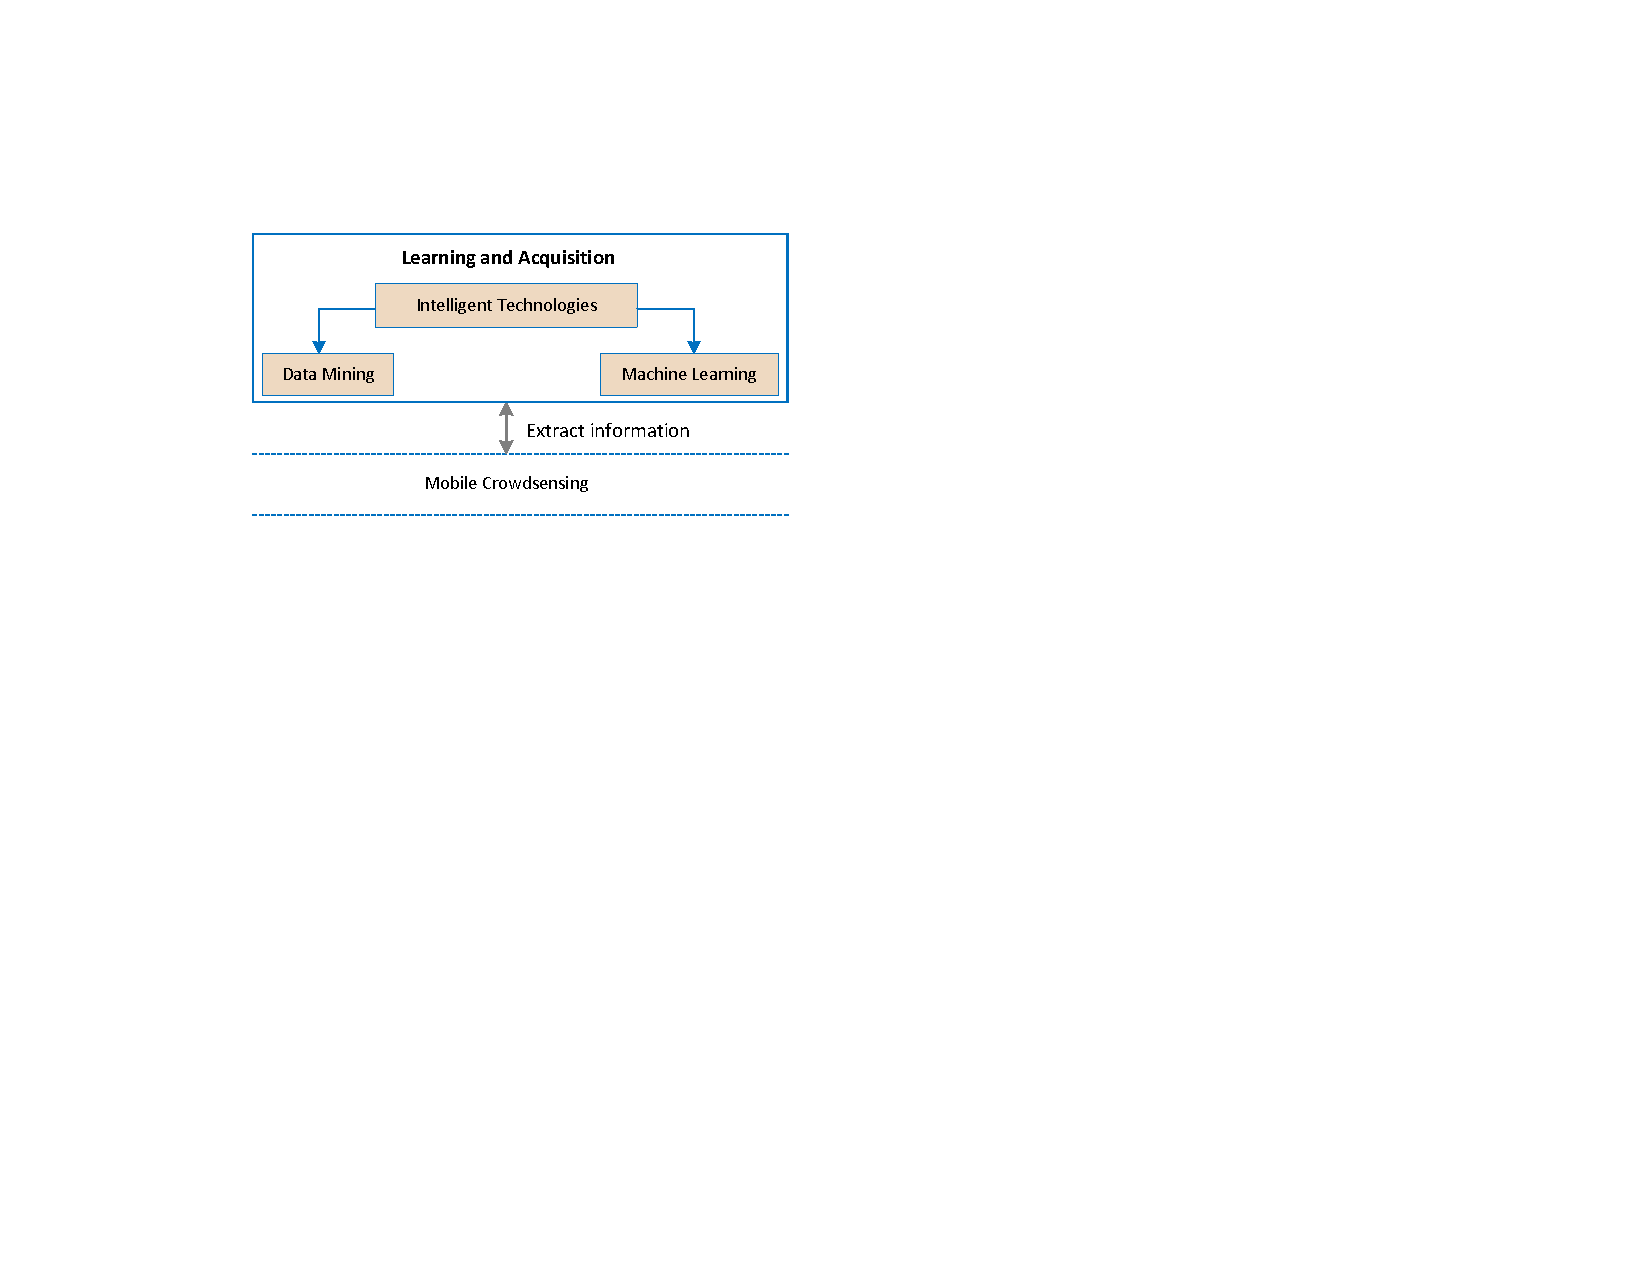
\includegraphics[width=0.65\textwidth]{Chap3-Fig2.pdf}
  \end{tabular}
  \caption{The learning and acquisition component.}
\end{center}
\end{figure}

The learning and acquisition component (Fig. 3.3) is responsible for collecting information that is to be used for social awareness component. The mobile crowdsensing component periodically reports to the learning and acquisition component observations from the sensors that can be used to understand users' activities. The learning and acquisition component extracts information from the mobile crowdsensing component using intelligent technologies such as data mining and machine learning.

Considering the unique characteristics of data from sensors, particularly its spatio-temporal behavior and existence of limitations related to the data collection and computational resources, there have been many research efforts to analyze the sensor data which build upon the general research in the data mining and machine learning community to deal with sensor data~\cite{ZLi2011}. In particular, the raw data from mobile crowdsensing component needs to be efficiently managed and transformed to usable information through these intelligent technologies. The lower layer (mobile crowdsensing) is responsible for sensing of user data. If we don't apply intelligent technologies, the collected data could be inaccurate and inconsistent. Therefore, preprocessing is needed using data mining and machine learning to integrate and get accurate data. Mining and learning are then required to be performed on the preprocessed data from the lower layers. These intelligent technologies operate on top of the data, enabling users to analyze it from different viewpoints that can be an input to the social awareness component.

\subsection{Social Awareness}\label{Chap3_02_03}
\esubsection{Social Awareness}
\begin{figure}[t]
\begin{center}
  \begin{tabular}{c}
  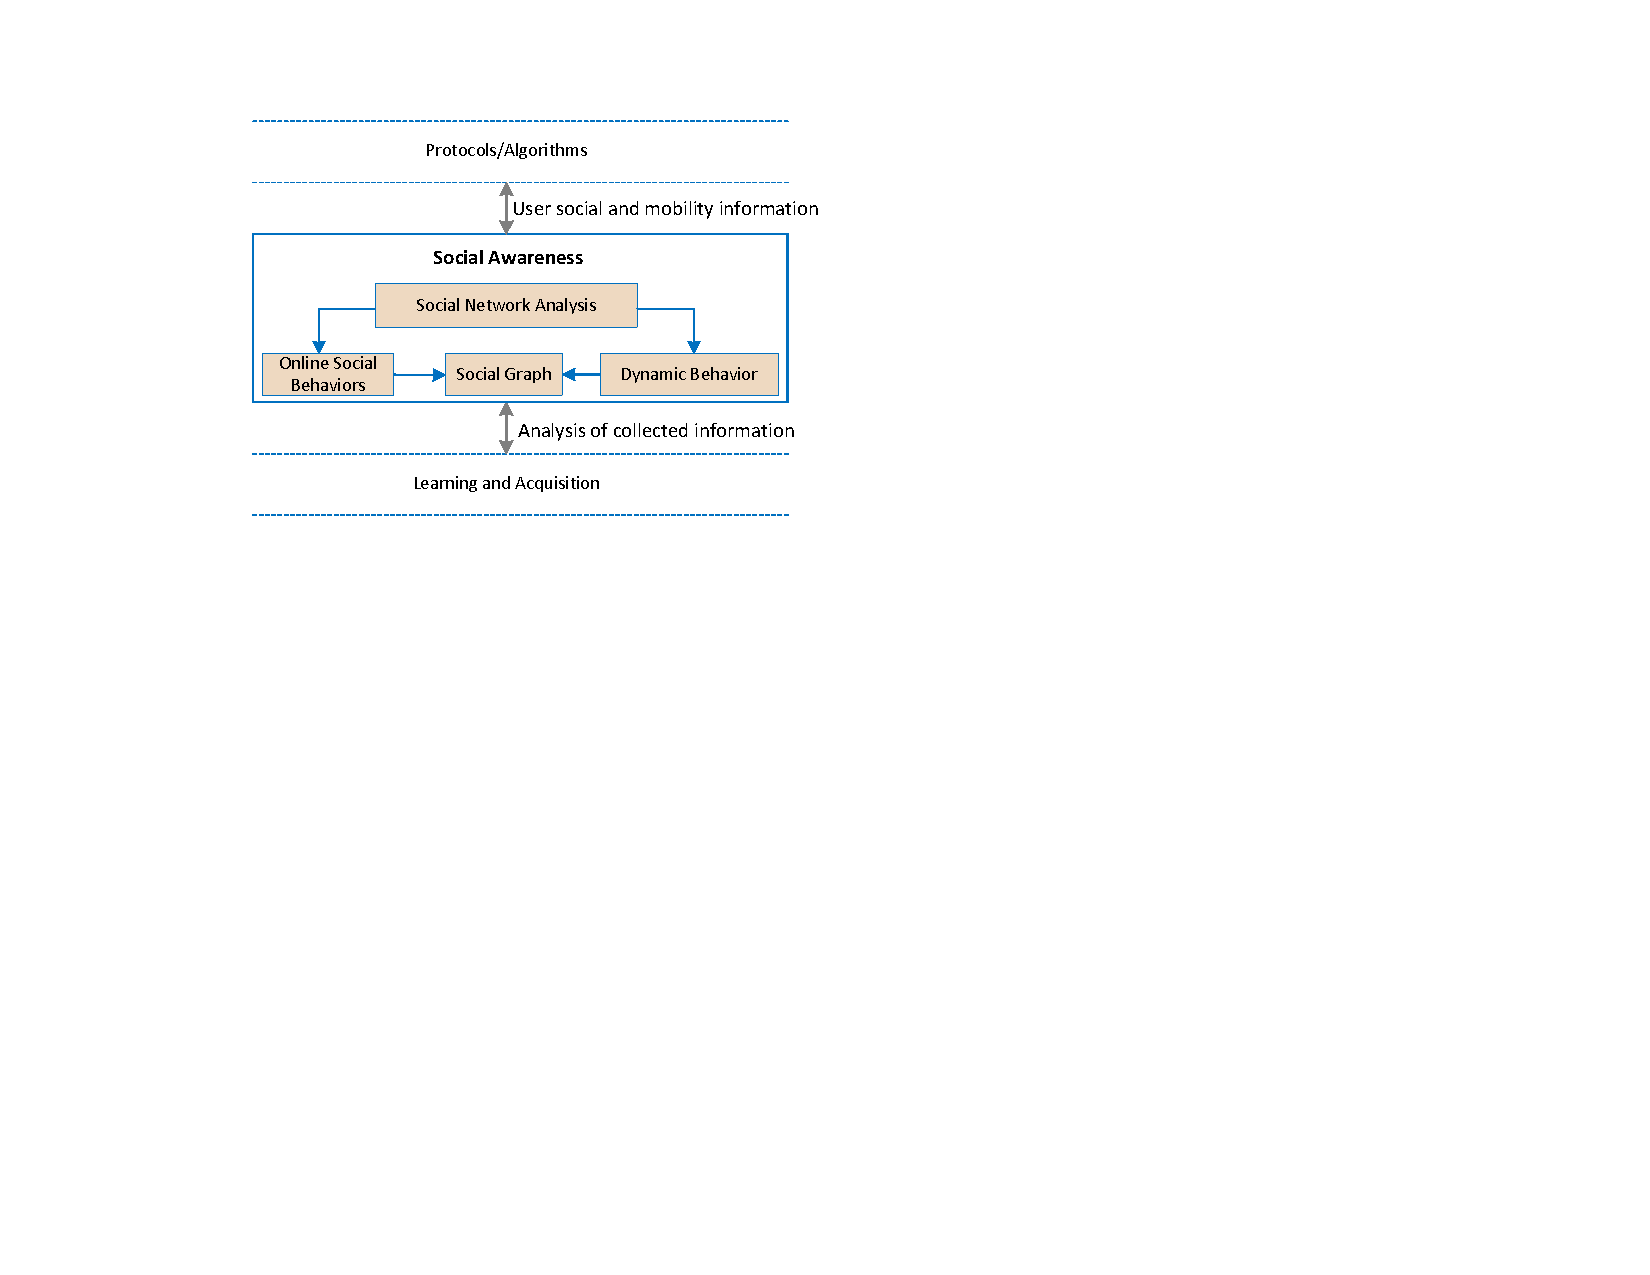
\includegraphics[width=0.65\textwidth]{Chap3-Fig3.pdf}
  \end{tabular}
  \caption{The social awareness component.}
\end{center}
\end{figure}

The social awareness component (Fig. 3.4) receives collected and processed data from the learning and acquisition component about activities of any user/community whose behavior is considered. This component then analyses the data using different social network analysis techniques and generated a social graph according to users online and mobility information which is the basis for the design of ASNET protocols/algorithms. Social Network Analysis (SNA) is the study of users and focuses on their interactions and relationships such as friendships and communications among users and the forms and consequences of these relationships~\cite{SWasserman1995}. The purpose of social network analysis is to understand the modeling, features and composition of social networks based on the user social information (online social behavior and dynamic behavior) and thus improves the social graph and social links contained within.

The user social and mobility information of a network can be observed when the graph structure of a social network is modeled and analyzed. An in-depth understanding of the graph organization of social networks is essential in order to assess the newly emerging socially-aware network paradigms and to comprehend the impact user social features have on the design of middleware protocols. The application of social graph based on online social behaviors (friendship, similarity, tie strength, etc.) and dynamic behaviors (mobility) to ASNTEs might result in the distinguishing the defects of the existing methods and help propose appropriate system models for this networking paradigm. Social graph structure is also helpful in highlighting the strength of relations/links such as strongly connected or weakly connected which gives an insight on how well the users in a network are connected. Once these social information are available from this component, it will be a valuable input to design the protocols/algorithms.

\subsection{Protocols/Algorithms}\label{Chap3_02_04}
\esubsection{Protocols/Algorithms}
The protocols/algorithms component is an important yet mostly neglected component of an ASNET middleware system. Due to its anywhere-deployment readiness (from lower level to high level), users' behavior in ASNETs will be significantly influenced by the deployment scenario. Factors such as online information and user mobility can greatly influence a user's behavior. Therefore, it's important to consider social awareness prior to designing protocols or algorithms for ASNETs. Understanding how a social graph is modeled at the social awareness component thus enables us to design protocols or algorithms based on users social features such as social behavior and mobility. The remaining part of this sub-section briefly explains some of protocols/algorithms under this component.

\subsubsection{Data Dissemination and Replication}\label{Chap3_02_04_01}
%\esubsubsection{Data Dissemination and Replication}
Data is an important element in any computer networks. In general wireless networks, but especially in ASNETs, data management turns to be an essential design problem and must address a new collection of challenges (e.g., coordinating actions with other nodes, limited processing speed, and storage capacity). Most existing mobility-assisted data access techniques in ad-hoc networking are designed to disseminate data to one or several particular destinations. Different from these works, middleware design for ASNETs should consider novel social-aware approaches and replication problem that allocates data among all moving users so that the users that are interested in this data item can get it easily either from their encountered friends or stranger nodes in the community. To facilitate efficient data dissemination and to ensure data availability in ASNETs, we must develop a potential and more realistic solution by optimizing jointly with the routing and forwarding challenges.

\subsubsection{Routing and Forwarding}\label{Chap3_02_04_02}
%\esubsubsection{Routing and Forwarding}
Recently, there has been a growing interest in the networking community for reliable routing solutions in ad-hoc networks that face problems like connectivity.
The following are the main forwarding approaches that meet the challenges of socially-aware networks.

\emph{Controlled flooding approaches}: Epidemic routing is a well-known technique for data forwarding; it maximizes message delivery and latency with a trade-off in resource consumption.

\emph{Social behavior-based approaches}: These approaches are largely devoted to understanding human mobility patterns and social network properties in wireless networks.

\emph{Swarm intelligence-based approaches}: Swarm intelligence approaches allow each flow to use its own optimization criteria based on its QoS requirements, rather than using a single metric for all flows.

The literature work of Xia {\it et al.}~\cite{FXia2013} shows that, consideration of controlled flooding techniques and social properties during the course of routing and forwarding protocol design to make better forwarding decisions have recently been studied extensively. One of the efficient social based protocols is BUBBLE Rap~\cite{PHui2011} that considers centrality and community metrics to effectively enhance delivery performance. However, little work has been done on applying swarm-intelligence based approaches. Although some works like, BEEINFO~\cite{FXia2014} made the beginning step in this direction, we believe that more work needs to be done regarding such questions as what classification bounds are in socially-aware networks with community-dependent or independent routings, and how it can be affected by a very challenging problem that influences the design of routing protocols such as congestion.

The performance evaluation of BUBBLE Rap shows that it has a similar delivery ratio, but much lower resource utilization than control flooding and other social-based forwarding protocols. The same way, BEEINFO outperforms control flooding and other social-based routing protocols with higher delivery ratio, less overhead and less hop counts. Therefore, we believe that rather than sticking to flooding and controlled flooding approaches, the combination of social-based (e.g. BUBBLE Rap) and swarm intelligence-based techniques (e.g., BEEINFO) may play a role on this front.

\subsubsection{Resource Management}\label{Chap3_02_04_03}
%\esubsubsection{Resource Management}
Resource management that encompasses a broad range of limited resources, such as CPU, bandwidth, memory, and energy, in the presence of social network dynamics is a very challenging problem. In many examples of resource management approaches, energy stands out as one of the most critical resources, as it depends on the remaining battery of the node and availability of recharging. Unlike the wired networks where bandwidth is abundant, bandwidth in ASNETs is scarce. Furthermore, the available bandwidth changes with time based on the context and traffic conditions such as mobility, weather conditions, network heterogeneity, and social behavior.

Although managing resources is a critical operation in wireless networks, and corresponding algorithms have been extensively studied in always active MSNs, little work has been done for ad-hoc social networks. Load balancing \& fairness is, to a large extent, related to energy~\cite{SManfredi2013}, and neither has been well studied under the broad spectrum of socially-aware networks. We believe that further research work on this topic is necessary to tackle various optimization objectives such as energy, bandwidth and load balancing \& fairness for ASNETs. A possible approach here is to assume that the other design challenges (i.e., routing and forwarding) are already fixed, so the load balancing \& fairness problem becomes a standalone problem. However, it would be more intriguing but challenging if the challenges are jointly optimized with social behavior for load balancing \& fairness.

\subsubsection{Reliability}\label{Chap3_02_05_04}
%\esubsubsection{Reliability}
Reliability is vital in the design of middleware for ASNETs to deal with sensitive data that are mostly applicable in this emerging network paradigm such as social relationships, activities and others. However, it is challenging to provide a simple yet powerful reliable technique while consuming relatively little resources. Unreliable (selfish or malicious) users in the network compromise data dissemination and routing by affecting data availability and integrity in wireless network systems. Most existing efforts on reliability algorithms with incentive techniques have only one objective; to handle malicious users and individually selfish users having the same degree of selfishness toward the other users. We believe that designing an incentive mechanism to detect and handle individually and socially selfish users differently (e.g., according to the context information, such as social information) would be of interest for future research. In addition to that, addressing the problem of reliability effectively will be beneficial for the handling of privacy and security problems. For instance, How do we balance the concern of privacy and security, by introducing a socially-aware system?

\section{Metrics}\label{Chap3_03}
\esection{Metrics}
Several evaluation metrics have been used for validating or evaluating middleware protocols in wireless networks. However, it seems to be there is no consensus on metrics used to evaluate different middleware protocols for ASNETs such as data replication, load balancing and reliability. Each chapter (chapters \ref{Chap4} - \ref{Chap6}) employs evaluation metrics which are highly relevant and appropriate to validate the protocols effectiveness and efficiency. These evaluation metrics are mostly defined quantitatively and qualitatively. Among the most widely used metrics are read cost and detection rates (true and false detection rates) for evaluating the effectiveness of middleware protocols (replication, load balancing and reliability), and overhead to assess its efficiency. These metrics are essential and should be employed in the evaluation of any ASNET middleware protocols.

In the remaining part of this section, we define and describe some of the metrics that can be applied for the comparison and evaluation of protocols considering more particular protocols such as data replication, load balancing and reliability. The metrics assess the performance of different protocol components of the middleware framework in terms of effectiveness and efficiency.

\subsection{Effectiveness}\label{Chap3_03_01}
\esubsection{Effectiveness}
Some of the metrics used to measure the effectiveness of the protocols/algorithms component of the framework are read cost, relocation cost, overall load and detection rate. What follows is short description about these metrics.\\
\emph{Read cost:} It represents the number of communities required to retrieve the data of a user and that of every neighbor of the same user. Replication as one of the protocols (see chapter \ref{Chap4}) have to attain reduced cost of read operations in the network, since it allows read operations to be conducted in the same community from the same storage space. Relocation cost is another important metrics for replication protocols. It represents the number of replicas relocated from one storage space to another in the network. \\
\emph{Overall load:} It specifies and measures the overall publications received by all brokers in the community. Here we are concerned about the employed number of brokers in the network since it influences the overall load.\\
\emph{Detection rate:} This metrics measures the effectiveness of reliability functionality in the framework. True and false detection rates are the most common metrics for assessing reliability/selfishness protocols and algorithms. True detection rate represents the amount of detected selfish users in the reliability model of the framework. False detection rate is of two types: false positive and false negative. False positive measures the amount of cooperative users mistakenly classified as selfish in the system. On the other hand, false negative detects the selfish users mistakenly classified as cooperative users. \\

\subsection{Efficiency}\label{Chap3_03_02}
\esubsection{Efficiency}
Accessibility, consistency, load distribution, overhead and network load balance are some of the prominent metrics used to quantify the efficiency of ASNET middleware protocols. \\
\emph{Accessibility:} This is an important metrics for a data management (replication and reliability) protocol. It represents the ratio of the number of successful access (query) requests to the number of all access requests issued throughout the network. A data replication protocol aims to increase the accessibility of data items in the network. Here, we are concerned on how the mobility of users in the network affects the accessibility of data in replication and reliability protocols. \\
\emph{Consistency:} Our concern with the assessment of existing replication protocols is the seemingly lack of importance placed on the consistency evaluation metrics of the replicas as they relate to capturing the state. The potential for stale information across the replicas seems to be very real, especially with ASNETs. We would like to see better assessment on the need to maintain consistent state across the replicas using the proposed framework.\\
\emph{Load distribution:} It measures the load distribution of every broker in a publish/subscribe data dissemination approach. How to ensure even distribution of load among brokers or storage spaces is a critical issue. Therefore, load balancing functionality of the framework can be assessed using this metrics as presented in \ref{Chap5_05_03}. \\
\emph{Communication overhead:} It measures the communication overhead exerted by the load balancing functionality of the ASNET middleware framework. \\
\emph{Network load balance:} It represents the ability of reliability protocols to balance traffic across users (including read and write operations) of network scenario without considering load balancing and fairness functionality of the framework.\\

\section{Applicability}\label{Chap3_04}
\esection{Applicability}
This research will apply to different areas of socially-aware networking environments that require support from a number of technologies such as mobile sensing, opportunistic sensing, mobile crowd sensing (MCS) and social network analysis. The developed ASNET middleware framework is meant to serve as a basis for designing and building new data dissemination/replication, routing \& forwarding, resource management and reliability protocols for ad-hoc social networks. The layer-based functionalities of the middleware system allow the designer and developers to choose the appropriate components from the sensing level to application level to activate based on factors such as the purpose and the deployment model of the ASNET applications. The framework will also aid in evaluating and comparing different middleware protocols for ad-hoc social networks.

Managing an event such as conferences for a smart community can be a frustrating matter for all planners, organizers and attendees. However, technological advances in wireless networks, the advent of new mobile devices and the proposal of efficient middleware protocols have made possible the development of mobile applications that can successfully support all parties. The ASNET middleware system framework and protocols proposed should operate in event guides particularly pervasive conference scenarios where data availability, balanced loads of storage spaces and cooperation are keys to maximizing data accessibility, network survival and users are assumed to be autonomous. Most importantly, it should apply to dynamic environments where network conditions change temporarily, requiring users to adapt the functionalities of their perspective middleware framework to optimize their operations.

\section{Summary}\label{Chap3_05}
\esection{Summary}
In this chapter we proposed a formal framework for ASNET middleware. We decomposed the framework into different components and discussed every component that builds a formal framework for ASNET middleware, the sub-component and functionalities of each component, and the relations among these components in terms of the data flow. The framework can be used to describe and design ASNET data management protocols. It also helps to compare protocols at different layers of the framework. We also presented metrics that can be used for quantitative and qualitative evaluation of designed protocols from an effectiveness as well as performance efficiency perspectives.


